\graphicspath{ {Background/Images/} }


\chapter{Generalized Word2Vec for Electronic Health Record Analytics}
\label{cha:background}

\section{Introduction}

In the previous chapter we introduced the field of electronic health record analytics and how this can be used to find new patterns in medical data. We discussed several methods such as querying, statistics, data mining, and artificial intelligence approaches. The methods we mentioned vary from simple to very complex. In the field of machine learning algorithms, a limited amount of research is done on EHRs, mainly using out-of-the box tools. Thus, the focus point of this thesis is: applying advanced machine learning algorithms to find patterns in EHRs. \\

In this chapter we introduce the field of time series as an analogy with medical data. Then we move on to machine learning concepts such as kd trees and neural networks. Both which are used in our approach to find patterns in time series. Then we explain the most important concept, namely Word2Vec. Later in this chapter we extend Word2Vec so we are able to apply it on medical data. \\
Note that in this chapter we give a first idea of the workings of our approaches. For a more detailed explanation on how our approaches are applied on medical data, we refer to chapter \ref{cha:implementation}. \\

The structure of this chapter is as follows. We start by explaining some background knowledge in section \ref{sec:bk}, such as time series and machine learning. We focus on basic concepts from machine learning and move on to neural networks. Crucial to understand our approach is the introduction of Word2vec in section \ref{sec:word2vec}. Then we introduce Deepwalk as an extension to Word2Vec in section \ref{sec:deepwalk}. Finally, we explain our own generalized Word2Vec approaches in section \ref{sec:gw2v}.


\section{Background Knowledge}
\label{sec:bk}

	\subsection{Time Series Analysis}
A time series consists of data points over a certain time period. We refer to this as a sequence of states. A state represents a data point and can differ from a single value to more complex representations like pictures. \\
The domain of time series analysis deals with extracting information or relations from a time series. It can have different goals like forecasting, classification, or exploratory analysis. \\

A medical history of a patient can be seen as a time series, namely a sequence of visits to the doctor. This means that methods which are applied to time series, can also be applied to medical data to find patterns. We focus on machine learning approaches which are applicable to time series.

	\subsection{Machine Learning}
Machine learning (ML) is a data-driven approach which aims to build a model which can be used to make predictions or decisions on new data \cite{ML:article}. Note that this model can be used to predict outcomes of time series. ML is carried out by algorithms which are able to learn models based on examples given by the designer. Based on the examples, machine learning provides $3$ types of approaches, namely supervised learning, unsupervised learning, and reinforcement learning. \\
Supervised learning is concerned with the learning task where there are examples given with their corresponding label (for example, a picture with the label dog). Unsupervised learning is similar to supervised learning only no labels are given. We will not go into reinforcement learning. \\
We can also classify the ML approaches according to the desired output of our model. Those main tasks consist of classification, regression, and clustering. Classification has a discrete output, namely the predicted label. Regression has a continious output, namely a predicted value. Clustering is typically an unsupervised approach which tries to find patters in the data based on a similarity measurement. \\
	
In the field of classification neural networks are used to achieve state of the art results. For regression, linear regression can be used. One of the most popular methods for clustering is k-means. 

	\subsection{K-nearest Neighbors}
	\label{sec:knn}
	
The k-Nearest Neighbors (knn) algorithm is a simple machine learning algorithm \cite{knn:article}. It will be used in our generalized Word2Vec approach. \\
When you are in a supervised context, you have several instances with labels. When you retrieve a new instance, you want to predict its label. Based on a predefined similarity measure (ex. Euclidean distance), you look for the $k$ labeled instances nearest to the new instance in a vector space determined by the features/variables. From those, you pick the most common label in the pool of the $k$ nearest instances. This label becomes your predicted label for the new instance (see figure \ref{fig:knn}).

\begin{figure}[!htb]
	\centering
	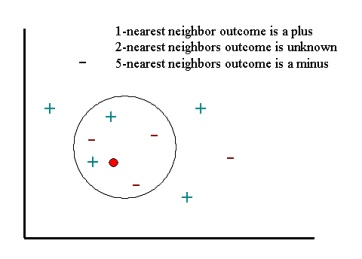
\includegraphics[width=0.6\textwidth]{knn.jpg}
	\caption{Representation on how the knn algorithm predicts a label for a new instance.}
	\label{fig:knn}
\end{figure}
	
	
	\subsection{K-dimensional Tree}
	\label{sec:kdtree}
	
A naive way to calculate the nearest neighbors for an element in a vector space, is by comparing all members with the new element and keep track of those distances. \\
A more efficient way is to use a k-dimensional tree (kd tree) \cite{kdtree:article}. In this section we explain the workings of this approach in more detail \cite{kdtreeIntro:atricle}. \\

A kd tree is a way of storing k-dimensional points. It is a binary tree where each node represents an element in the vector space. The node also contains information on how the tree is split up in terms of hyperplanes in the vector space. It keeps track of the plane it is split on and the left and right sub tree. In figure \ref{fig:kdtreeSplit} you can see an example on how a simple kd tree is constructed and how it splits up the x,y plane. In the top figure, the splitting plane is not mentioned. The bottom figure shows that it is the $y=5$ plane for the $[2,5]$ and $x=3$ for $[3,8]$. \\
	
\begin{figure}[!htb]
	\centering
	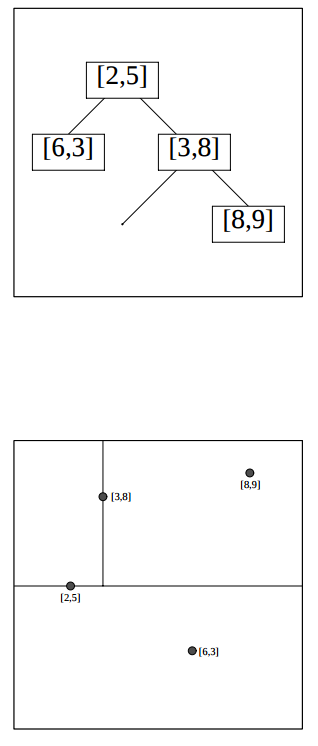
\includegraphics[width=0.4\textwidth]{kdtreeSplit.png}
	\caption{Representation on how a binary kd tree splits up the plane  \cite{kdtreeIntro:atricle}}
	\label{fig:kdtreeSplit}
\end{figure}


Now that we can construct the kd tree, we can use it to find the nearest neighbor for a certain input point. We start with the root node and go down the kd tree depth-first. At each node, the algorithm goes to the left or right depending on whether the input is less or greater than the current nodes value on the splitting plane. Once the algorithm reaches a leaf node, it marks this leaf node as the current nearest neighbor. \\
The algorithm unwinds the recursion of the tree, performing the following steps at each node:
\begin{itemize}

\item If the current node is closer than the current best, then it becomes the current best.
\item It checks whether there is the possibility of points closer to the input point on the other side of the splitting plane. It makes a hypersphere around the current node with a radius equal to the current nearest distance. 
\begin{itemize}
\item If the hypersphere crosses the splitting plane, there could be a closer point on the other side. This means the algorithm will move down the other branch of the current node.
\item If the hypersphere does not cross the splitting plane, the whole other branch can be skipped.
\end{itemize}
\end{itemize}

This algorithm is easily extended to find the k-nearest neighbors by keeping track of the k current bests. Kdtree has a complexity of $\mathcal{O}(\log{}n)$ compared to $\mathcal{O}(dn)$ with $d$ the dimension of the search space for a naive knn implementation.
	
	\subsection{Neural Networks}
	
A neural network is a machine learning approach based on biological neural networks. It can be used to find patterns in and make predictions about time series. Those time series can be speech, videos, medical data, \ldots \\
Besides being used in finding patterns and making predictions, it is also used in Word2Vec. This is explained in section \ref{sec:word2vec}.


		\subsubsection{Perceptron}

The basic component of a neural network is the perceptron \cite{perceptron:article}. A perceptron takes multiple binary inputs and has a single binary output (see figure \ref{fig:perceptron}). Each input has a corresponding real numbered weight $w_j$. The output is decided by the following equation: \\

\begin{equation} 
output =
  \begin{cases}
    0       	& \quad \text{if } \sum_j w_jx_j \leq \text{ threshold}\\
    1  		& \quad \text{if } \text{if } \sum_j w_jx_j > \text{ threshold}\\
  \end{cases}
\end{equation}
	
\begin{figure}[!htb]
	\centering
	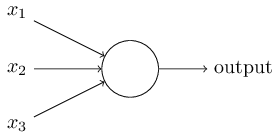
\includegraphics[width=0.4\textwidth]{perceptron.png}
	\caption{Simple representation of a perceptron \cite{NNintro:online}.}
	\label{fig:perceptron}
\end{figure}

The equation above, represents an activation function. The function retrieves certain inputs, and has an output between $0$ and $1$. There are several activation function possible in a perceptron as we will discuss later on. \\
We can build a network by connecting multiple perceptrons (see figure \ref{fig:multiplePerceptrons}). By building these networks, more complex decisions can be made. The reason for this, is that once there are at least $3$ layers of perceptrons (and non-linear activation functions), the network can find non-linear relations between the input and output \cite{nnNL:article}. \\

\begin{figure}[!htb]
	\centering
	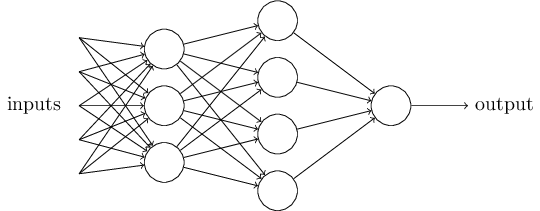
\includegraphics[width=0.8\textwidth]{multiplePerceptrons.png}
	\caption{More complex network connecting multiple perceptrons \cite{NNintro:online}.}
	\label{fig:multiplePerceptrons}
\end{figure}


		\subsubsection{Terminology}

Now that we have seen how a general network is constructed, we introduce at some further vocabulary. \\
In figure \ref{fig:networkArch}, we see a four-layer network. As specified in the figure, we call the first layer the input layer, the last layer the output layer, and the layers in between hidden layers. Sometimes a multiple layer network is referred to as multilayer perceptrons or MLP. 

\begin{figure}[!htb]
	\centering
	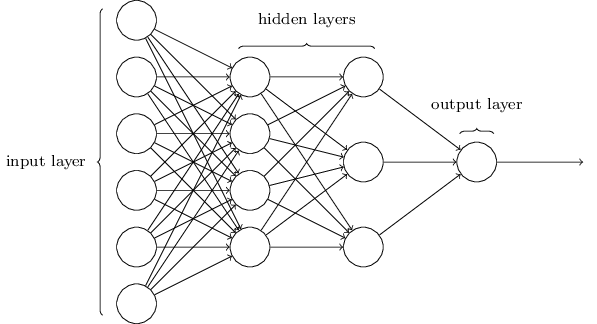
\includegraphics[width=0.8\textwidth]{networkArchitecture.png}
	\caption{General vocabulary of a multilayer network \cite{NNintro:online}.}
	\label{fig:networkArch}
\end{figure} 	

We use $w^l_{jk}$ to denote the weight corresponding to the connection between the $k^{th}$ node in the $(l-1)^{th}$ layer and the $j^{th}$ node in the $l^{th}$ layer. We use $b^l_j$ for the bias of the $j^{th}$ node in the $l^{th}$ layer and $a^l_j$ for the activation of the $j^{th}$ node in the $l^{th}$ layer. See figure \ref{fig:termNN}. \\

\begin{figure}[!htb]
	\centering
	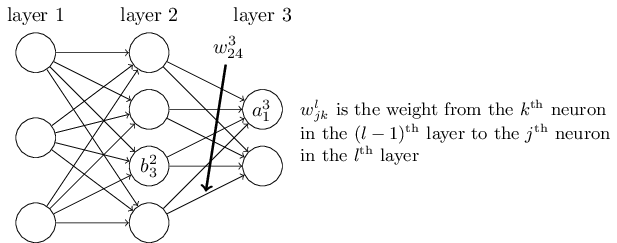
\includegraphics[width=0.8\textwidth]{termNN.png}
	\caption{Visual representation of the terminology for a neural network \cite{NNintro:online}.}
	\label{fig:termNN}
\end{figure} 

\noindent We remove the indexes for the node numbers which results in the following vector notations:

\begin{equation} 
a^l = \sigma (w^la^{l-1}+b^l) = \sigma (z^l)
\end{equation}	


		\subsubsection{Training a network}
		
To train a neural network, we input an example with a known output (or also called label). The network calculates a certain output based on the current weights, which is also called a forward pass. When this output is incorrect, it should be possible to adjust the weights to the effect that the network has as output the correct label, which is also called the backward pass. Note that the change in weights, should only affect the output in a limited way (see figure \ref{fig:smallChange}). The reason for this is that otherwise all the previous inputs could be labeled incorrectly. So, the concept of training a neural network means: adjusting the weights in a way that the behavior of the network is stable for the previous examples but such that the current example is labeled correctly. \\

\begin{figure}[!htb]
	\centering
	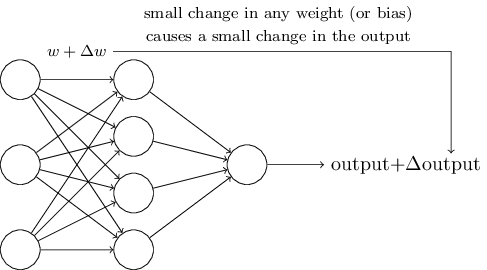
\includegraphics[width=0.8\textwidth]{smallChange.png}
	\caption{Change in weights, with respect to the impact on the output \cite{NNintro:online}.}
	\label{fig:smallChange}
\end{figure} 

To achieve this effect, sigmoid neurons were adopted instead of perceptrons. A sigmoid neuron has the same basic behavior as a perceptron, but has as activation function the sigmoid function instead of the step function, see figure \ref{fig:sigmoid}. A sigmoid function is easy to work with as it is bounded, easy differentiable, and monotonic \cite{transfer:article}. \\
We also introduce a bias $b$ which we ignored in the explanation of the perceptrons. Weights can now range between $0$ and $1$ while the output is calculated with $\sigma(w*x+b)$ where $\sigma$ is the sigmoid function. This results in the following formula: 

\begin{equation} 
output = \sigma(w*x+b) = \frac{1}{1+exp(-\sum_j w_jx_j-b)}
\end{equation}

\noindent We approximate $\Delta output$ in function of $\Delta w_j$ and $\Delta b$:

\begin{equation} 
\label{eq:costFunction}
\Delta output \approx \sum_j \frac{\partial output}{\partial w_j}\Delta w_j + \frac{\partial output}{\partial b}\Delta b
\end{equation}

\noindent Because of the linearity and the smoothness of the sigmoid function, it is now easier to choose changes for the weights and biases to achieve a correct output. By adjusting the weights, we train our network to achieve a higher accuracy on the examples seen.

\begin{figure}[!htb]
	\centering
	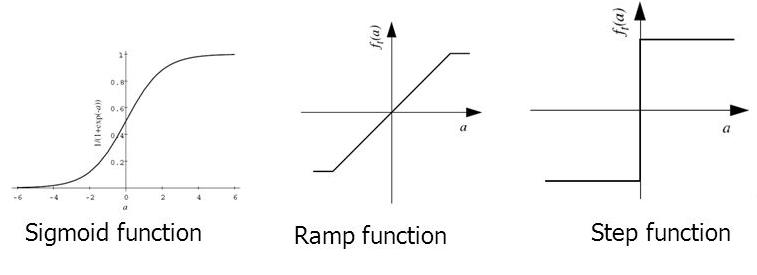
\includegraphics[width=0.7\textwidth]{sigmoid.jpg}
	\caption{Different activation functions.}
	\label{fig:sigmoid}
\end{figure} 
		
	\subsection{Backpropagation}
	
To train a neural network, we define a function which has to be minimized. This function is called the cost function. Backpropagation aims to efficiently calculate the gradient of the chosen cost function with respect to the individual weights and biases \cite{bp:article}. Backpropagation can be used in combination with an optimization technique called gradient descent. Based on the gradient, gradient descent updates the weights of the neural network and minimizes the cost function \cite{NNintro:online}.

		\subsubsection{Cost Function}
		
As mentioned before, backpropagation aims to calculate the gradient of the cost function $C$ with respect to each weight and bias. For a neural network, we can choose any cost function which fulfills the following mentioned criteria. \\
The first one is that it needs to be possible to write it as a summation over cost functions for individual training examples. Secondly, it needs to be derivable. And lastly, the cost function is a function of the activations of the last layer. \\
An example cost function which we will use is:

\begin{equation} 
C = \frac{1}{2}\sum_j (y_j - a^L_j)^2 \text{ with L the last layer}
\end{equation}

		\subsubsection{Fundamental Equations}

Backpropagation has 4 equations. The equations allow us to calculate the error and the gradient of the cost function. These are used to adjust the weights and biases based on the gradient descent algorithm. \\

First we calculate the error for each node in the last layer. The error is based on how fast the cost function is changing as a function of the $j^{th}$ output activation and on how fast the activation function $\sigma$ is changing at $z_j^L$:

\begin{equation} 
\delta^L_j = \frac{\partial C}{\partial a^L_j} \sigma'(z_j^L)
\text{ with }
z_j^L = \sum_k w^L_{jk}a^{L-1}_k+b^L_j \text{ and } \sigma' the derivative of \sigma
\end{equation}

\noindent This can be written as a neat vector equation:

\begin{equation} 
\delta^L = (a^L-y) \circ \sigma'(z_j^L)
\end{equation}

\noindent The next equation explains why the algorithm is called backpropagation. The equation calculates each layer's error vector based on the next layer and so propagates the error back through the layers:

\begin{equation} 
\delta^l = ((w^{l+1})^T\delta^{l+1}) \circ \sigma'(z_j^L)
\end{equation}

\noindent With those 2 equations we calculate the error in each layer of the neural network. Those errors can be used to calculate the derivatives of the cost function with respect to the weights and the biases:

\begin{equation} 
\frac{\partial C}{\partial w^l_{jk}} = a^{l-1}_k \delta^l_j.
\end{equation}

\begin{equation} 
\frac{\partial C}{\partial b^l_j} = \delta^l_j.
\end{equation}

\noindent When the derivatives are calculated, we can apply the gradient descent algorithm and update the weights and biases accordingly. This process represents the learning of a neural network.


\section{Word2Vec}
\label{sec:word2vec}

\subsection{Motivation}

In this section, we explain Word2Vec \cite{w2vOriginal:article} from a linguistic point of view. Word2Vec lies at the basis of our generalized extension which can be applied to medical data. Word2Vec is introduced in 2015 by the Google Brain Team and is currently an active research field. \\ 

In natural language processing tasks, a good representation of words helps algorithms perform better. Word2Vec learns a representation which maps words to vectors in a low-dimensional space compared to the vocabulary size. In this representation, context-similar words are mapped close to each other in the new vector space. The new representation is called a 'word embedding'. 
We could say in an informal way: a linguistic background is learned and can be used by other algorithms to increase their performance. \\
A sentence can be seen as a time series of words. Therefore it is possible to generalize Word2Vec to medical data (which is also a time series). As we apply a generalized Word2Vec to medical data, we call this a disease embedding. \\

\subsection{Neural Networks}

When the Word2Vec algorithm is trained using the Skip-Gram model (see section \ref{sec:skipgram}), one relies on a lookup table. This table contains the mapping of words to their vector representation. This lookup table can be found by training a 2-layer neural network with as cost function the function described in \ref{eq:w2vCost}. The training can be done with backpropagation for example. \\
The trained 2-layer neural network can be placed in front of another neural network \cite{w2vNN:online}. The former converts the words to their vector representation and feeds it into the latter neural network. It is empirically shown that the results of the neural network can be improve by putting the lookup table in front of it \cite{w2vOriginal:article}. As mentioned before, in a way, you offer background knowledge to the neural network.

\subsection{Skip-Gram Model}
\label{sec:skipgram}

There are two main models used for Word2Vec, namely Continuous Bag-of-Words (CBOW) and the Skip-Gram model. \\
The former predicts a word based on a given context (ex. predict Paris when capital France is given). The latter does the inverse of this approach \cite{w2vModels:article}. Empirical results have shown that the Skip-Gram model tends to perform better on larger datasets \cite{w2vReason1:online} and establishes a better representation for infrequent words \cite{w2vArchive:online}. In medical data infrequent diagnoses may be important along a patient's trajectory. For those reasons, we choose use the Skip-Gram model in the rest of our work. \\

Learning a Word2Vec representation of a corpus $Text$ with the Skip-Gram model proceeds as follows. \\
Based on given words $w$ and their contexts $c$, we set the parameter $\theta$ of the probability $p(c|w;\theta)$ to maximize equation \ref{eq:skipgramMax}. The probability $p(c|w;\theta)$ is indeed the probability of a context occurring with word $w$ as mentioned before. We refer to section \ref{sec:parameterization} for more information about $\theta$.

\begin{equation} 
\label{eq:skipgramMax}
\arg \max_{\theta} \prod_{(w,c) \in D} p(c|w;\theta)
\end{equation}

\noindent with $D$ the set of all word-context pairs we extract from the corpus.


\subsubsection{Establishing word-context pairs}

Given a sequence of words, we define their context based on n-grams \cite{w2vNgram:article}. In figure \ref{fig:ngram}, n-grams are shown for the sentence "This is a sentence". 

\begin{figure}[htbp]
	\centering
	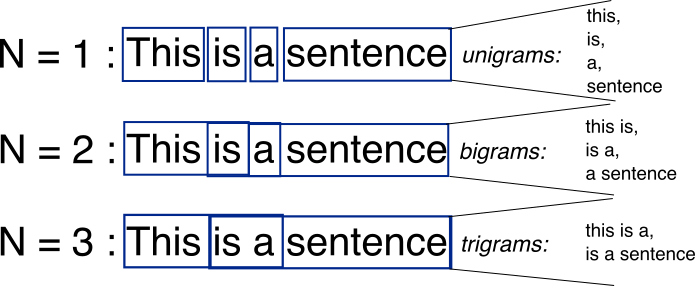
\includegraphics[width=0.8\textwidth]{ngram.png}
	\caption{Explanation of n-gram \cite{w2vNgram:online}}
	\label{fig:ngram}
\end{figure} 

For the n-gram, we define the context of a word $w_t$ as $w_{t \pm n}$. A larger $n$ typically results in more specific contexts for training examples and thus can lead to a higher accuracy, if there is enough data to back this up. Indeed, if there are not enough cases handling those specific contexts, the correlation between the word and his context is less statistically significant.


\subsubsection{Parameterization by $\theta$}
\label{sec:parameterization}

We start by rewriting the conditional probability using a soft-max function \cite{softmax:article}:

\begin{equation} 
p(c|w;\theta) = \frac{e^{v_c*v_w}}{\sum_{c' \in C}e^{v_{c'}*v_w}}
\end{equation}

\noindent where $v_c$ and $v_w$ are vector representations for context $c$ and word $w$, and $C$ is the set of all available contexts. Because we want to maximize $p(c|w;\theta)$, it means that $\theta$ represents the parameters $v_{c_i}$ and $v_{w_i}$. Computing the optimal parameters is very expensive because you need to calculate this over all contexts $c' \in C$. We also switch from product to sum by taking the logs:

\begin{equation} 
\arg \max_{\theta} \sum_{(w,c) \in D} \log p(c|w;\theta) = \sum_{(w,c) \in D} (\log e^{v_c * v_w} - \log \sum_{c' \in C} e^{v_{c'}*v_w})
\end{equation}

\subsubsection{Negative Sampling}

To compute the hyperparameters $\theta = \{v_c, v_w\}$ using the Skip-Gram model more efficiently, we introduce negative sampling \cite{w2vExplained:article}. \\
Instead of calculating $\sum_{c' \in C}e^{v_{c'}*v_w}$ over all contexts, we make a set $D'$ which consists of randomly sampled word-context pairs. With this new set, we remove the costly term $\sum_{c' \in C}e^{v_{c'}*v_w}$ and replace it with $\sum_{(w,c) \in D'}e^{v_{c'}*v_w}$: 

\begin{equation} 
\label{eq:w2vCost}
\arg \max_{\theta} \sum_{(w,c) \in D} \log p(c|w;\theta) = \sum_{(w,c) \in D} (\log e^{v_c * v_w} - \log \sum_{(w,c) \in D'}e^{v_{c'}*v_w})
\end{equation}

Informally, while not ensuring that if words appear in the same context, their vectors are closer together than all the other word vectors, we only make sure they are more similar than a several vectors chosen randomly. Negative sampling makes the Skip-gram model usable in terms of computation.

\section{DeepWalk}
\label{sec:deepwalk}

DeepWalk is an approach for applying Word2Vec on graph-structured data \cite{deepwalkMain:article}. \\
DeepWalk generates random sequences based on the graph structure. Word2Vec is then applied on those sequences to learn a good vector representation for the vertices. We can say that it is an extension to the Word2Vec approach by allowing it to be applied to more varied types of data. \\

In figure \ref{fig:dwAlgo}, we see an overview of the DeepWalk algorithm. It consists of two parts. \\
First, in line 6, a random walk generator generates for each vertex $v_i$ of the graph $G$, a random walk of length $t$. It will do this $\gamma$ times but the order $\mathcal{O}$ in which the vertices are traversed, is randomly chosen for each pass. With those walks, a sequence of vertices is generated. \\
Secondly, in line 7, this sequence is used for Word2Vec with the Skip-Gram model For this SKip-Gram model we use $w$ as the size for the n-grams (also called window size) and $d$ as the dimension of the new vector space. This process is explained in section \ref{sec:word2vec}.

\begin{figure}[!htb]
	\centering
	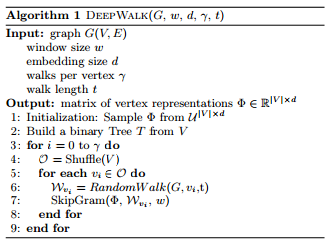
\includegraphics[width=0.7\textwidth]{dwAlgo.png}
	\caption{Overview of the DeepWalk algorithm \cite{deepwalkMain:article}}
	\label{fig:dwAlgo}
\end{figure} 

\section{Generalized Word2Vec Approaches}
\label{sec:gw2v}

In this section we explain our approach on how to find patterns in EHRs using Word2Vec techniques. For this, we formulate a generalized Word2Vec approach tailored to the context of learning disease embeddings.

\subsection{Data representation}

Before we can start with explaining how Word2Vec can be applied on EHR data, we introduce our data representation. \\
The medical history of a patient is a time series of EHR events. On certain timestamps, an EHR event is available containing the medical info (diagnose, lab result, \ldots) about that patient. We denote this EHR event the vector $m^p_t$, with $p$ a patient number and $t$ a timestamp. This means that each patient has a sequence of vectors $s^p = m^p_t, m^p_{t+1}, m^p_{t+3}, \ldots$ Each vector $m^p_t$ contains certain values depending on the event. It can contain values of the event's time, demographics, blood pressure, diagnoses, and others (see figure \ref{fig:matrixPatient}. 

\subsection{Generalized Word2Vec}

As explained in section \ref{sec:word2vec}, Word2Vec is typically applied to a large text corpus containing a large amount of sentences. After applying this method, an embedding is found that represents words in a new vector space. In this vector space the relationship between words is shown by the distance of the words from each other. \\

A medical dataset containing EHRs from different patients can be seen as a large text corpus. It contains patients, each with an EHR (or a sequence of EHR events) $s^p$, which is equivalent to one sentence. The set $\{s^p\}$ is considered as a corpus of sentences made up of words $m^p_t$. Each vector $m^p_t$ is removed from the features which uniquely link it to the patient like the timestamp or patient identifier, we call this trimmed vector $m$. This is to make the link to words. Different sentences can contain the same words in that vectors $m$ can be part of different sequences. \\

With the above, it is possible to apply Word2Vec on corpus $\{s^p\}$. We call this a generalized Word2Vec approach. From this, we can learn an embedding for the vectors $m$. The embedding shows the relationships between the vectors $m$ with others in the sequences $\{s^p\}$ based on their contexts. \\
Others have explored other analogies with for example protein sequences (BioVec) \cite{protvec:article}. Note that with BioVec, their vectors $m$ are still the same as words as they are both one-dimensional.


\subsection{K-Nearest Neighbors Word2Vec}
\label{sec:knnWord2Vec}

A problem with embeddings established for a certain dataset is that because Word2Vec builds a lookup table, there is the possibility that a certain instance is not present in the lookup table and therefore no representation can be found for this instance. \\ 
Since we are working in the context of a generalized Word2Vec approach, where instances are represented by complex objects like vectors $m$, the possibility of this happening increases. For example, an EHR event can be a multi-dimensional vector where each feature has a broad range of values. Compared to a word, which is a one-dimensional vector with as range all words in a dictionary, an EHR event has more possible combinations. \\

Therefore we introduce a k-Nearest Word2Vec approach whereby we extend our generalized Word2Vec approach with a knn feature (see section \ref{sec:knn}). To our knowledge, this has not been done before. We use a kd tree method to find the knn, see section \ref{sec:kdtree}. \\

After the training of a Word2Vec model, we have learned a lookup table which maps a known vector $v_{old}$ to his new vector representation $v_{new}$. When a not-yet-seen vector $v_{unknown}$ needs to be mapped to his $v_{new}$, a normal Word2Vec is not capable of this. \\
In our approach, we find the k-nearest neighbors of the $v_{unknown}$ from the representations $v_{old}$ in the lookup table. We then take the new representations of the knn, and combine them using a weighted average to estimate the new representation $v_{new}$ for $v_{unknown}$. This way our approach is capable of finding a representation for complete new instances. \\

In short: we look for the knn of the $v_{unknown}$ from all the known vectors in the lookup table in their original representation $v_{old}$. Based on the found knn, we take a weighted average of the representations $v_{new}$. This weighted average is the $v_{new}$ for the $v_{unknown}$.

\subsection{Generalized Deepwalk}
\label{sec:genDW}

Deepwalk starts from graph-structured data and is therefore not directly applicable to EHR data. One advantages of Deepwalk that it provides a method which can control a fixed amount of sequences. When the EHR dataset becomes very large, it would take a considerable amount of time to train a Word2Vec model. \\

Therefore it would be interesting to transform the EHR data into a weighted graph structure. The weights are based on the frequency of diagnoses following each other in all the sequences. \\
After the graph transformation, the amount of weighted random walks can be limited to create a smaller set of sequences based on the original dataset. Those sequences can be used to train a Word2Vec model faster as there is fewer data. The same logic from the previous two sections is applicable to generalize DeepWalk from words to more abstract objects.

\subsubsection{Graph Transformation}

In algorithm \ref{alg:graphTrans}, we explain the graph transformation. \\
To execute the graph transformation, we start by looping over each sequence from $\{s^p\}$. For each sequence we keep track of the previous seen element and the current element. From those $2$ elements we make $2$ vertices connected by an edge in line 6. \\
We add this edge to the current graph in line 7:

\begin{itemize}

\item If the edge between those two vertices already exists in the graph, we increase the weight of the existing edge by one.

\item If the edge does not exist in the current graph, but one of the vertices does exist, we add a new edge between the existing vertex and the newly added vertex. The weight of this new edge equals to one.

\item If the edge does not exist and the two vertices also do not exist in the graph, we add them all to the graph.

\end{itemize}

\begin{algorithm}
\caption{Graph Transformation}
\label{alg:graphTrans}
\begin{algorithmic}[1]

\State \textit{output: } Graph
\ForAll{Sequence in Sequences} 
	\ForAll{Element in Sequence} 
		\State PreviousElement
		\State CurrentElement
		\State Edge = MakeEdge(PreviousElement, CurrentElement)
		\State Graph.addEdge(Edge)
	\EndFor
\EndFor

\end{algorithmic}
\end{algorithm}

\section{Conclusion}
In this chapter we discusses general machine learning concepts and focused on Word2Vec. We conclude that Word2Vec is used to find good representation of words based on their context. It also causes that similar words will be close to each other in this new representation. \\

With the concepts explained, we introduced our generalized Word2Vec approaches with as goal to find patterns in EHRs. We extended Word2Vec so that it can handle more abstract objects than words, namely vectors representing an EHR event. We also extended Word2Vec to find a representation for a new instance based on knn. We also generalized DeepWalk to reduce the training time of Word2Vec on large medical datasets.



%%% Local Variables: 
%%% mode: latex
%%% TeX-master: "thesis"
%%% End: 
